Si les jeux vidéo sérieux commencent à être connus du grand public et leur impact reconnu, ceux pour la santé ne sont pas encore assez nombreux ni assez largement acceptés. Mon travail de stage s'inscrit en réponse à cette constatation : il s'agit de proposer une méthode de conception de jeux vidéo pour la santé qui permettrait une simplification ou une amélioration de la conception de tels jeux. Proposer plus de jeux  thérapeutiques et/ou des jeux avec un impact santé de plus grande qualité contribuerait à améliorer leur diffusion et leur reconnaissance. Pour ces raisons, il était ainsi primordial de parfaire ma connaissance des différents domaines concernés.

Cette partie présente le résultat de mes recherches, des techniques et outils existants et comporte des notions importantes à connaître pour la conception de serious games pour la santé.

%****************** Subsection 1 : jeux vidéo
%% PART 1 : JEUX VIDEO
\subsection{Jeux Vidéo}
Durant mon stage, j'ai ainsi voulu comprendre pourquoi et comment un jeu vidéo est bon, quels en sont les mécanismes ou bien encore quels facteurs vont retenir le joueur. 

	%%Définition d'un Jeu 
	\subsubsection{Définition d'un Jeu}
Le jeu vidéo est un média participatif en pleine extension et de plus en plus largement accepté et plébiscité par la population. \\Dans sa définition, un jeu vidéo est une extension du jeu au monde numérique en utilisant les technologies informatiques. Il s'agit donc en amont de bien comprendre ce qu'est un jeu. \\Dans son travail d’analyse, Juul\cite{Juul05} donne une synthèse qui regroupe les points partagés par toutes les définitions existantes~:
\begin{quotation}
A game is a rule-based formal system with a variable and quantifiable outcome, where different outcomes are assigned different values, the player exerts effort in order to influence the outcome, the player feels attached to the outcome, and the consequences of the activity are optional and negotiable. 
\end{quotation}
\paragraph{Points clefs \\}
Les 6 points clefs identifiés par Juul sont :
\begin{itemize}
	\item les règles
	\item le résultat quantifiable variable
	\item la valorisation du résultat
	\item l’effort du joueur
	\item l’attachement du joueur au résultat (identifié par Gendler comme Alief, 2009)
	\item des conséquences négociables.
\end{itemize}

		\subsubsection*{Pratique et consommation des jeux vidéo}
Le jeu vidéo est un média récent qui trouve ses origines dans le début de la seconde moitié du XX$^{eme}$ siècle. D'abord majoritairement accessibles sur des bornes d'arcade, les jeux vidéo se sont progressivement répandus avec la commercialisation de consoles de salon. Selon une étude commandée par le Centre National du Cinéma et de l'image animée\href{http://www.cnc.fr}{(CNC)}, c'est près de 60\% de la population française qui jouaient à des jeux vidéo au cours de l'année 2011\cite{Cnc11}. L'âge moyen des joueurs était alors de 34,7 ans et cette population constituée de 54,1\% d'hommes fin 2011\cite{Cnc11}. L'arrivée de la console Wii et de jeux orientés plus casuals\footnote{Se dit d'une personne ne jouant à des jeux vidéo que de manière occasionnelle. Peut aussi se dire d'un jeu dont la cible sont des joueurs occasionnels.} a permi en France une meilleure diffusion du média au sein de la population, qui accepte de plus en plus de se livrer à cette activité. Contrairement à ce que l'on pourrait croire, notamment à cause de leur méconnaissance des nouvelles technologies et du jeu vidéo plus spécifiquement, les seniors se prêtent aussi volontier à la pratique de ce loisir numérique. C'est une constation que nous avons pu vérifier par nous-même lors de nos différentes sessions de tests au centre hospitalier de Lapeyronie et dans une maison de retraite à Lille, mais aussi dans différentes lectures qui seront détaillées ci-après.
	
		\subsubsection*{Propriétés des jeux vidéo}
En 1984, [Driskell and Dwyer]\cite{Dris84}réalisent un premier état de l'art et trouvent que plusieurs caractéristiques des jeux vidéo peuvent influer sur les propriétés d'apprentissage et de motivation : des objectifs spécifiques, un challenge, de la fantaisie et du mystère. Ils théorisent qu'une augmentation de la motivation produit une augmentation de l'attention et mène à une meilleure mémorisation des acquis (connaissance déclarative) et une focalisation de l'attention (stratégie cognitive).\newline
[Malone et Lepper, 1987] mentionnent le challenge, la curiosité, le contrôle et la fantaisie comme caractéristiques intégrantes des jeux vidéo. Selon [de Felix et Johnson , 1993], les jeux sont composés d'éléments visuels dynamiques, d'interactions, de règles et d'objectifs. Puis [Thiagarajan, 1999] affirme que le conflit, le contrôle, la terminalité et l'artifice sont les quatre éléments nécessaires d'un jeu. En 2001, [Garis and Ahlers, 01] donnent 39 descripteurs qui seront réduits à 12 pour ne garder que les paramètres statistiquement les plus significatifs pour renforcer la sensation de "game-like". \\ Finalement en 2002, [Garris et al] proposent un sous-ensemble de tous ces attributs qui seront considérés commes les paramètres de jeu clefs de l'apprentissage~:
\begin{itemize}
	\item la fantaisie
	\item les règles
	\item la stimulation sensorielle
	\item le challenge
	\item le mystère
	\item le contrôle
\end{itemize}

\paragraph{}En 2009, [Wilson et al]\cite{Wils09} partent de l'ensemble de paramètres de [Garris et al] pour enrichir le modèle avec de nouveaux paramètres qui leur semblent avoir un impact sur l'apprentissage.
Les tableaux \ref{game_attributes_one} et \ref{game_attributes_two} indiquent et décrivent ces douze attributs.

\begin{figure}[htbp]
	\centering
	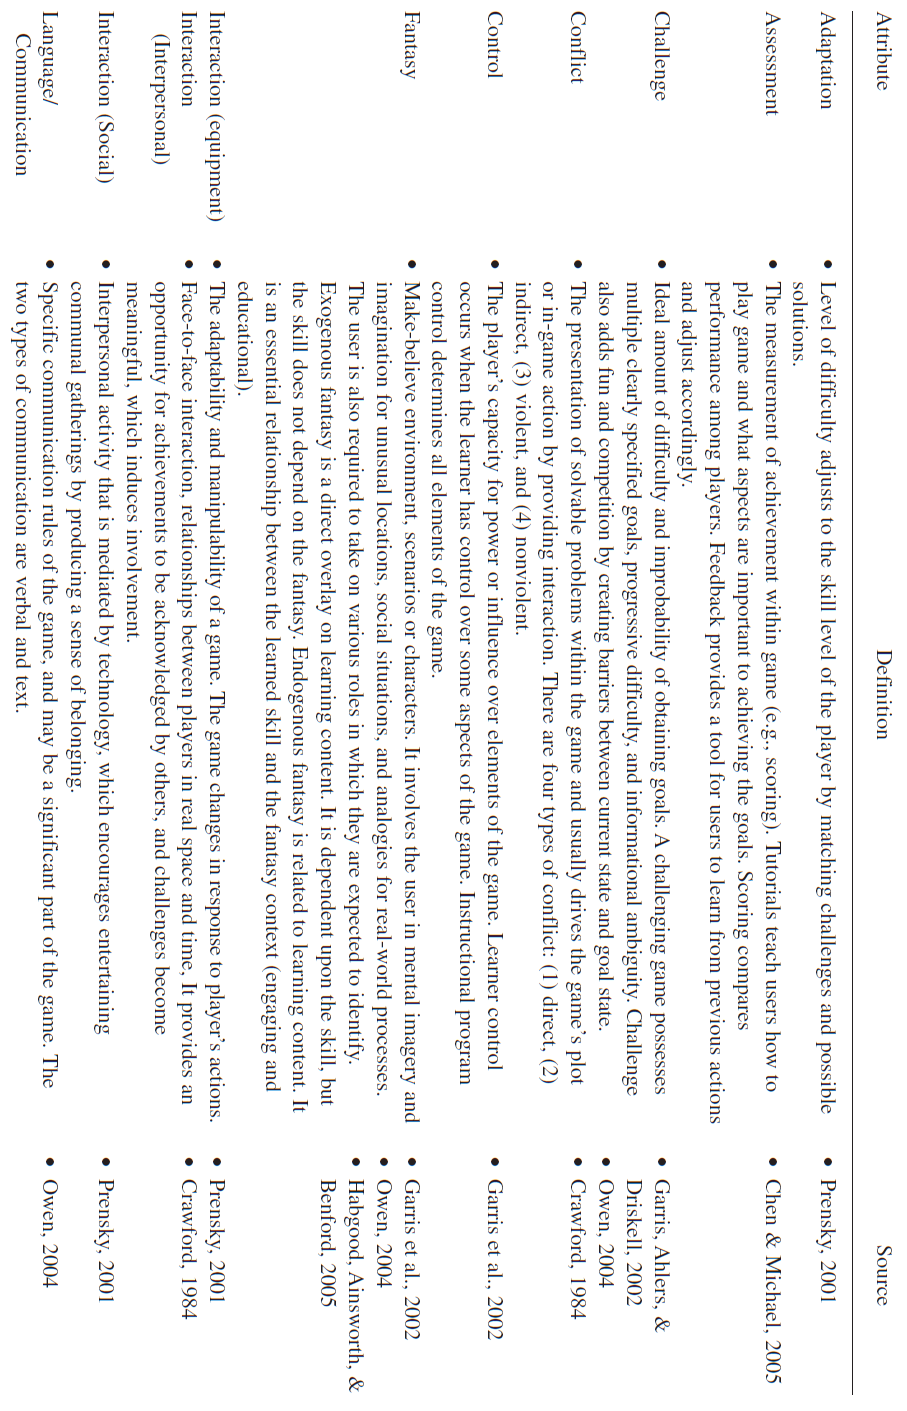
\includegraphics[width=\linewidth, height=\textheight ]{images/game_attributes_one}
	\caption{Propriétés des jeux vidéo et leur définition. (1/2) \cite{Wils09}}
	\label{game_attributes_one}
\end{figure}
\begin{figure}[htbp]
	\centering
	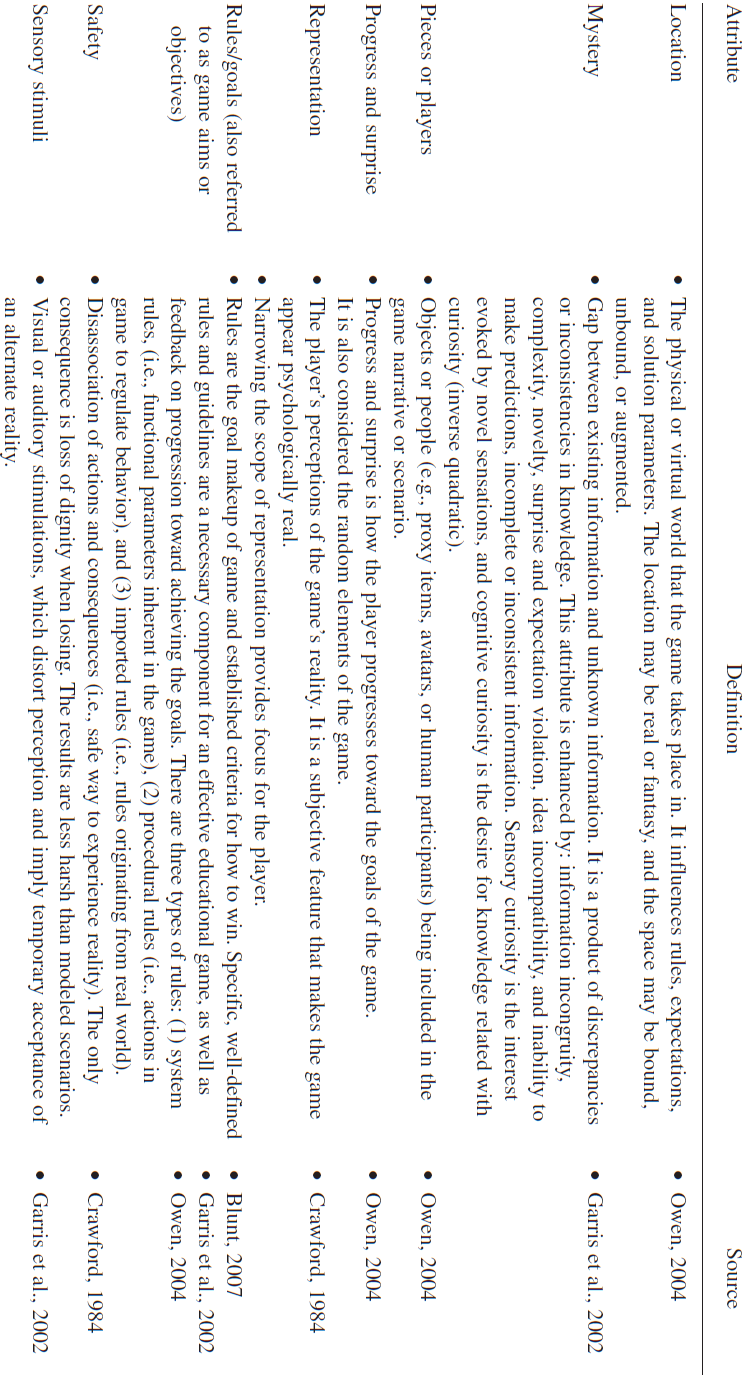
\includegraphics[width=\linewidth, height=\textheight ]{images/game_attributes_two}
	\caption{Propriétés des jeux vidéo et leur définition. (2/2) \cite{Wils09}}
	\label{game_attributes_two}
\end{figure}	

	%% Jeux vidéo et schéma comportementaux
	\subsubsection{Jeux vidéo et schémas comportementaux}
Pour expliquer l'attrait croissant de la population envers les jeux vidéo, il peut être intéressant de se tourner du coté des théories comportementales. Carl Rocray \cite{Rocr09} explique qu'en dépit de ses origines technologiques récentes, le jeu vidéo entretient d’anciens schémas de comportements, et cette influence est subtile. C’est le propre du jeu de nous divertir, non seulement de nos tracas réels, mais aussi de son influence sur nous pendant que nous jouons. Cette influence est évidente à travers le lien entre plaisir et apprentissage : l’effort diminue si on a du plaisir à le faire, et on peut même en oublier que nous apprenons.

\paragraph{}On se rend compte que la plupart des jeux vidéo peuvent être classés selon leur gameplay en ce que l'on appelle des types de jeux. Parmi les grands types connus, on retrouve par exemple les jeux d'action, les jeux de stratégie ou encore les jeux de simulation sportive. On trouvera en \href{types_jeux}{annexe} une liste plus complète de ces types de jeux vidéo classés en fonction de leur gameplay. \\

Il est intéressant de constater le lien entre les différents schémas comportementaux basiques et les types de jeux mettant en place des mécaniques stimulant nos instincts primaires [Rocray, 09]\cite{Rocr09}.

\paragraph{}
		\paragraph{Survie \\ \quad}
«Éliminer ou être éliminé». C’est la base de la majorité des jeux vidéo et probablement aussi le comportement le plus simple. Même les jeux de sports ou de cartes entretiennent cet instinct primaire, bien qu’il soit surtout manifeste dans les jeux de tir (\emph{Doom}, \emph{Gears of War}), les jeux de combats (\emph{Tekken}, \emph{Street Fighter}) et les «platformers» (\emph{Mario Bros}, \emph{Assassin’s Creed}).
		\paragraph{Gestion \\ \quad}
Il s’agit surtout de gestion de ressources, mais aussi d’équipement quand celui-ci est limité. Une bonne gestion permet habituellement de mieux survivre (meilleures ressources, équipement adéquat), ce qui nécessite une planification et une organisation stratégiques. On retrouve ce comportement dans les jeux de simulation (\emph{SimCity}, \emph{Civilization}), de «Real Time Strategy» (\emph{Warcraft}, \emph{Starcraft}) et ceux qui visent un certain réalisme (\emph{Arma}, équipement limité dans \emph{Resident Evil}).
		\paragraph{Responsabilisation d’autrui \\ \quad}
Ce comportement fait appel à une sorte d’instinct parental où nous devons assurer la survie d’un autre joueur ou le bien-être d’un avatar virtuel qui nous ramène en fait à nous-même. Il est d’abord présent dans les jeux de simulation (\emph{The Sims}, \emph{Tamagotchi}) et ceux de coopération (\emph{Army of Two}, \emph{Left 4 Dead}).
		\paragraph{Résolution de puzzles \\ \quad}
Mystères à résoudre (\emph{Myst}), problèmes de logique faisant appel à nos capacités cognitives (\emph{Brain Challenge}), voire comment empiler des formes (\emph{Tetris}) ou aligner des couleurs (\emph{Bejeweled}), il s’agit toujours de trouver la solution la plus efficace à un problème donné.
		\paragraph{Réflexes et dextérité \\ \quad}
La plupart des jeux font appel à cet instinct également lié à la survie.
Surtout lié à la coordination «oeil-main» et à la précision d’actions souvent rapides (voir entre autres les «Quick-Time Events»), il est aussi lié à la maîtrise d’un outil, c’est-à-dire la manette de jeu. On le retrouve dans les jeux de rythme (\emph{Guitar Hero}, \emph{Rock Band}), mais aussi dans les jeux de Survie cités plus haut et tous les jeux de sports.
		\paragraph{Système de récompenses \\ \quad}
La grande majorité des jeux vidéo utilise ce système de la carotte au bout du bâton pour diriger les actions du joueur. Il est donc étroitement lié à la motivation et à la gratification de comportements donnés. Voir entre autres \emph{Little Big Planet} et \emph{Diablo}, ainsi que la mode assez récente des Trophées, Succès et autres «Achievements».
		\paragraph{Système d’améliorations \\ \quad}
Une autre mécanique liée à la Survie et à la courbe de difficulté des jeux. En bref, il s’agit de devenir plus fort pour défaire des adversaires toujours plus forts. C’est la base des «Role-Playing Games» (\emph{World of Warcraft}, \emph{The Elder Scrolls}) et de certains jeux de «Shooter» (pour améliorer ses armes).

		\paragraph{}
Il est probable que d’autres comportements soient ainsi entretenus par le médium vidéo-ludique. Les sept types de mécaniques décrites ci-haut montrent néanmoins comment les jeux vidéo nous font répéter d’anciens schémas de comportement.

		\subsubsection*{Autres aspects du comportement pour la motivation du joueur}
			\paragraph{\emph{Conditionnement} \\ \quad}
Un autre aspect du jeu vidéo est sa capacité à encadrer, voir conditionner, le joueur pour lui donner envie de continuer à jouer (Voir la théorie du conditionnement par Pavlov). Bien sur, en règle générale, on cherche à ce que le joueur joue pour le plaisir, et non dans un quelconque but de conditionnement. Pour cela, le jeu va soumettre le joueur à un ensemble de stimuli de récompenses (incrémentation du score, gain d’un bonus, débloquer un niveau, feedback, etc.) lorsqu’il réalise une action positive, ou de punition (baisse du score, perte du niveau, de points de vie, etc.) lors d’erreurs. En choisissant ces ensembles de stimuli positifs et négatifs, on réussit à faire accomplir intuitivement aux joueurs ce que l’on espère qu’ils fassent.

\paragraph{}
Ces ensembles de stimuli constituent une sorte de récompenses à l’accomplissement des différentes actions du joueur. Les règles du Game Design nous enseignent qu’un jeu vidéo est constitué d’un ensemble de boucles de jeu situées à trois niveaux : micro (scène), moyen (scène et level) et macro (jeu). Ce sont les boucles OCR+M : Objective, Challenge, Reward et Means.
\begin{itemize}
	\item Objectif : état qui décide si la boucle est terminée ou non
	\item Challenge : pourquoi le joueur ne peut pas atteindre directement l’objectif
	\item Reward : récompense donnée au joueur une fois l’objectif atteint
	\item Means : moyens mis à disposition pour atteindre l’objectif
\end{itemize}
La mise en place d’objectifs a donc lieu a trois niveaux afin de toujours garder la motivation du joueur.

\paragraph{}
Plutôt que de parler de conditionnement, on peut plutôt d’association d’idées, concept sur lequel se base le conditionnement simple. Le jeu ne cherche en effet qu’à guider le joueur dans le but de le rendre autonome en lui apprenant les règles qui régissent son gameplay. Plutôt que de dire explicitement l’impact de chaque action, le jeu va souvent faire sentir au joueur ou lui faire comprendre l’impact de celle-ci, notamment par le biais des feedbacks. Libre au joueur de s’adapter ou non, sa marge de liberté étant différente d’un jeu à l’autre.\\
Un jeu comme Pong associe directement le fait de rater une balle avec celui de donner un point à l’adversaire (et donc de rapprocher le joueur de la défaite) alors que renvoyer la balle et passer l’adversaire sera clairement montré comme une action positive. Bien qu’il reste libre de ne pas chercher à renvoyer les balles et tromper l’adversaire, sa marge de liberté reste cependant limitée par le potentiel d’action et les règles du jeu : il pourra par exemple essayer de faire durer l’échange le plus longtemps possible ou chercher à ne gagner qu’avec un seul point d’avance, mais n’obtiendra aucune récompense pour cela de la part du jeu, qui n’a pas pensé à cette association d’idées. A l’inverse un jeu plus riche comme Fable ou Minecraft sera beaucoup moins binaire qu’un simple “bien / pas bien”.

	%%State of Flow
	\subsubsection{L'état de flux ou expérience optimale}
Le state of flow ou état de flux, fut originellement décrit par Csikszentmihalyi\cite{Csik88} dans les années 80 bien qu'il utilisa déjà ce terme dans ses recherches précédentes\cite{Csik75}. C'est l'état dans lequel une personne peut se trouver, proche de l’extase (dans le sens “se trouver à coté de”) complètement immergée dans ce qu'elle fait, dans un état maximal de concentration. Cette personne éprouve alors un sentiment d'engagement total et de réussite. Dans cet état, on est alors hyper compétent, naturellement, inconsciemment dans ce qu’on est en train de faire : musique, sport, travail, jeux, lecture, etc. Cet état est commun chez les personnes exerçant une activité répétitive et/ou demandant de gros efforts physiques ou psychiques. On est comme détaché de son corps, que l’on voit agir tout seul. On est alors capable d’accomplir des choses qu’on serait incapable de réaliser consciemment de manière contrôlée. S’il n’est pas interrompu, cet état d'expérience optimale peut durer une dizaine ou une vingtaine de minutes.

\paragraph{}
L’état de flux est l’une des raisons pour lesquelles on joue aux vidéo [Murphy, 2011]\cite{Murp11}. Leur but est de divertir en jouant sur la motivation du joueur, ce qui est lié au flow state. Le jeu, au moyen d’une balance entre compétences et challenge, maintient la vivacité d’esprit du joueur, avec une motivation importante et une attention forte[Rutledge, 2012]\cite{Rutl12}. Être dans cet état de flux permet donc au joueur une meilleure expérience de jeu augmentant son ressenti et son souhait de continuer à jouer[Chen, 07]\cite{Chen07}. Pour rentrer dans cet état de grâce, les deux états d’esprit les plus proches sont l’excitation et le contrôle, le flow state se trouvant à l’intersection de ces deux noeuds. On peut donc essayer de mettre le joueur dans ces états là si on cherche à stimuler ce flow state.

\begin{figure}[h!]
	\centering
	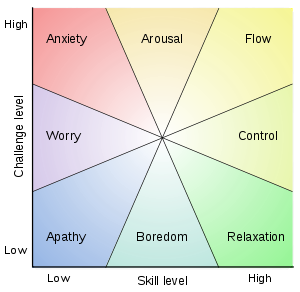
\includegraphics[width=9cm]{images/state_of_flow.png}
	\caption{Positionnement entre les humeurs et l'état de flux [Csikszentmihalyi, 1997]\cite{Csik97}}
	\label{state_of_flow}
\end{figure}

\paragraph{}
Csikszentmihalyi identifie les caractéristiques de l’état de flux~:
\begin{enumerate}
   \item prédispositions ou caractéristiques propices pour atteindre cet état~:
         \begin{itemize}
            \item des objectifs clairs et précis
            \item équilibre entre difficulté de la tâche et compétences de l’acteur (joueur)
            \item l’activité est en soi une source de satisfaction (amusante ou pour laquelle le joueur est impliquée)
         \end{itemize}
   \item conséquences et caractéristiques~:
   	\begin{itemize}
            \item hyperfocus, concentration exacerbée sur une action précise
            \item perte de la conscience de soi
            \item perception du temps modifiée
            \item rétroaction immédiate : prise de conscience de l’action effectuée, pour ajuster les suivantes
            \item sentiment de contrôle de la situation
	\end{itemize}
\end{enumerate}


%****************** Subsection 2 : Serious games et Theories comportementales
	\subsection{Jeux sérieux}
Les jeux vidéo se révèlent être un outil dont l’impact peut dépasser la simple portée ludique. 
		\subsubsection*{Définitions}
		\label{sggt}
On notera bien la différence entre les serious games conçus spécifiquement avec un objectif sérieux des autres aspects sérieux que peuvent revêtir les jeux vidéo et logiciels éducatifs. 

\paragraph{•} \emph{Les logiciels ludo-éducatifs} ont pour objectif de présenter
sous forme de jeu vidéo un contenu éducatif, en insérant des séquences ludiques avec des défis et des récompenses [Natkin, 09\cite{Nat09}]. Parmi les plus connus, on pensera notamment à \emph{Adibou} et \emph{GCompris}.

\paragraph{•}\emph{Les serious games} se proposent de profiter du ressort ludique du jeu vidéo pour servir volontairement un objectif sérieux distinct. Jeux éducationnels, commerciaux, idéologiques ou d’entraînement font partie de cette famille des jeux sérieux. D’un point de vue thérapeutique, il est possible de les utiliser afin de rendre le travail de réhabilitation ou de remise en forme plus motivant pour le patient en combinant les aspects ludique et thérapeutique.

\paragraph{} Natkin différencie les logiciels ludo-éducatifs des jeux vidéo éducatifs qui sont  une des formes des \glspl{sg}. Ces derniers exploitent les mécanismes d’immersion et d’apprentissage utilisés dans les jeux vidéo pour améliorer certaines compétences et connaissances du joueur\cite{Nat09}.

\paragraph{•}\emph{Le serious gaming} est la dérive de l'utilisation d'un jeu vidéo classique ludique dans un objectif sérieux distinct et non prévu dans la conception du jeu. Il est par exemple possible de jouer à un jeu vidéo permettant de conduire des véhicules dans une ville (les séries \emph{GTA} ou \emph{Driver} par exemple) dans le but de réviser son code de la route. C'est une forme de gameplay émergeant, c'est-à-dire une situation complexe rendue possible par les mécanismes de base mis en place dans le jeu, issu de l'appropriation de celui-ci par les joueurs.

\paragraph{•}\emph{L'apprentissage tangentiel} représente les connaissances ou compétences acquises par le joueur lors de ces sessions de jeu de manière non volontaire et non directement prévues par les concepteurs du jeu. Cela peut être le fait de développer ses connaissances linguistiques en jouant à un jeu non traduit, de développer son vocabulaire ou d'acquérir des connaissances dans un jeu ayant un thème particulier (vocabulaire militaire ou d'arsenal dans un jeu de guerre, connaissances théologiques dans un jeu sur l'Égypte ou la Grèce antique par exemple).

		\subsubsection{Serious games et théories comportementales}
Les jeux vidéo sérieux se présentent comme un potentiel médiateur dans la modification des habitudes comportementales en permettant d’inclure des connaissances pratiques dans un modèle ludique apprécié. Il est possible d’y mettre en place des procédures de changement comme l’établissement d’objectifs ou la modélisation et le développement de compétences dans un environnement attrayant, significatif et immersif [Baranowski et al, 2008]\cite{Bara08}. \\
Les jeux vidéo promeuvent les interactions sociales et d’apprentissage [Wideman et all, 2008], créent un environnement où les actions du joueur ont un effet [Gee, 2004]\cite{Gee04} , encouragent la résolution de problèmes [Gee, 2004]\cite{Gee04} et renforcent la compréhension en créant des situations de réflexion ou en aidant le joueur dans ses objectifs [Gee, 2004]\cite{Gee04}. Enfin, les jeux sérieux pour la santé sont fait pour distraire le joueur tout en l’éduquant, en l’entrainant ou en changeant ses comportements [Stokes, 2005]\cite{Stok05}.

		\subsubsection*{Théories comportementales}
Le comportement est la résultante d’influences multiples, rendant ainsi souvent les personnes réfractaires au changement [Baranowski, Lin \& al, 1997]\cite{Bara97}. Le comportement doit alors être considéré comme un mécanisme complexe découlant de l’enchaînement de plusieurs étapes. Ainsi, plutôt que de chercher à impacter directement le comportement, les experts comportementaux valorisent une action sur ces facteurs intermédiaires, appelés médiateurs. Changer ces médiateurs permet de changer le comportement [Baranowski, Lin \& al 1997]\cite{Bara97}.
\paragraph{}Plusieurs grandes théories comportementales existent~:
\begin{itemize}
	\item la théorie d’inoculation comportementale [McGuire, 1961]
	\item la théorie socio-cognitive [Bandura, 1986]
	\item la théorie de l’auto-détermination [Ryan \& Deci, 2000]
	\item la théorie de l’immersion [Green \& Brock, 2000]
\end{itemize}

\paragraph{}De ces théories, l’on peut alors identifier un certain nombre de ces facteurs médiateurs tels que : l’immersion, l’attention, l’auto-régulation, le développement de compétences, la motivation interne et externe, l’autonomie ou encore le sentiment de compétence. La science du comportement fournit aussi des techniques qui facilitent le changement comportemental, et propose d’utiliser ces facteurs dans les média de divertissement tel que le jeu vidéo.\\
Le modèle : "Elaboration Likelihood Model" [Petty \& Cacioppo, 1986] soutient ainsi que des personnages crédibles, attrayants et sympathiques sont plus susceptibles d’être persuasifs que les autres et peuvent donc servir d’intermédiaires pour véhiculer un message. \\
La théorie d’inoculation comportementale [McGuire, 1961] met en garde contre une possible contre-productivité en identifiant et en réfutant les menaces potentielles à l’accomplissement des objectifs du changement désiré.\\
La théorie socio-cognitive [Bandura, 1986] préconise l’établissement d’objectifs et le développement de compétences comme paramètres importants dans le changement comportemental.\\
Enfin, les théories socio-cognitive [Bandura, 1986] et d’auto-détermination [Ryan \& Deci, 2000] mettent toutes deux l’accent sur l’importance du feedback pour guider et mettre en forme le comportement durant le processus de changement.	

	\subsubsection{Jeux sérieux thérapeutiques}
Dans notre contexte, l’aspect sérieux recherché du jeu est la réhabilitation motrice ou la rééducation physique du joueur. Ces objectifs sont indiqués par des thérapeutes, médecins ou kinés, notamment dans le cadre de réhabilitation de personnes hémiplégiques ou souffrant de douleurs lombaires. L’intérêt du jeu vidéo est alors de proposer un environnement de réhabilitation plus agréable et de faciliter l’acceptation des travaux de rééducation par le patient grâce aux éléments de gameplay. Le jeu peut permettre un plus grand volume de travail de la part du patient car celui-ci sera plus enclin à les réaliser dans le cadre du jeu sérieux. Surtout, le jeu sérieux augmente la répétition de mouvements, ce qui améliore l'état physique du joueur-patient. L’objectif à terme est donc d’améliorer les résultats de l’objectif thérapeutique.


%****************** Subsection 3 : Difficulté
	%%PART 3 : LA DIFFICULTE
\subsection{Difficulté}
Dans son livre \emph{La cigale : jeux, vie et utopie}, le philosophe Bernard SUITS indiquait : \begin{quote}{“Jouer consiste à tenter volontairement de surmonter des obstacles inutiles”}.  \end{quote}
		
	\subsubsection{Définition et propriétés}
La difficulté s’inscrit comme l’un des principes de base dans la création d’un jeu vidéo, et l’un des mécanismes pourvoyeurs de plaisir principaux de celui-ci. Il n’y en en effet pour un joueur rien de plus frustrant qu’un jeu à la difficulté inexistante ou à l’inverse tout bonnement injouable de part sa difficulté excessive. \paragraph{}

Dans sa thèse, Guillaume Levieux [Levieux, 2011]\cite{Levi11} propose de définir la difficulté d’un jeu vidéo comme l’effort fourni par le joueur pour atteindre ses objectifs. La difficulté d’un jeu n’est pas une donnée stable et suit un processus qui doit être en constante évolution. Le niveau du joueur varie en effet au fil du jeu, du fait de son expérience et de son apprentissage, et la difficulté doit donc s’adapter. 
La difficulté n’est donc en fait pas une propriété du jeu mais la valeur de la relation entre le jeu et le joueur. Or en jouant, le joueur progresse, découvre l’univers du jeu et parfait sa connaissance de la mécanique du jeu, devient capable d’heuristiques pour prévoir les conséquences de ses actions, augmente ses capacités de coordination oculo-manuelle et sa vitesse de réalisation des actions. La difficulté est donc variable, et tend à diminuer au cours du temps. La figure \ref{evolution_difficulte} illustre l'évolution de la difficulté d'un jeu au cours du temps.\\
Notons que le niveau du joueur peut aussi varier à la baisse, si il ne joue pas au jeu pendant un certain temps par exemple. \\

G. Levieux précise donc dans sa définition de la difficulté, qu’il est important de prendre en compte son aspect relationnel avec le joueur et introduit alors les notions de difficulté absolue et relative~:
	\begin{itemize}
		\item la difficulté absolue d’un jeu décrit l’effort que doit fournir un joueur type, aux capacités statiques, pour atteindre les objectifs que son gameplay propose. 
		\item la difficulté relative d’un jeu décrit l’effort que doit fournir le joueur, dont les capacités évoluent tout au long du jeu, pour atteindre les objectifs que son gameplay propose.
	\end{itemize}
\paragraph{}Pour maintenir la difficulté relative du jeu, il est donc nécessaire d’augmenter la difficulté absolue du jeu en fonction de l’évolution des capacités du joueur.

\begin{figure}[!htbp]
	\centering
	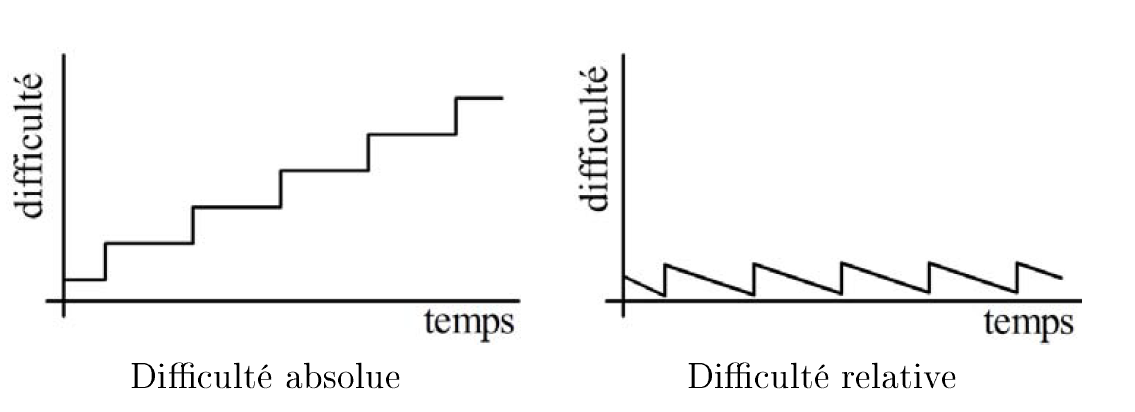
\includegraphics[width=11cm]{images/evolution_difficulte.png}
	\caption{Evolution de la difficulté d'un jeu au cours du temps}
	\label{evolution_difficulte}
\end{figure}

\paragraph{}La difficulté augmente si l’on resserre les contraintes et délais d’exécutions des actions, si on ajoute de nouveaux éléments qui augmentent la complexité du système ou si l’on découvre une nouvelle partie de l’univers demandant ainsi une appréhension du système plus étend. A l’inverse, la difficulté tend à baisser pour le joueur qui travaille son habileté, ou enregistre le mécanisme de nouveaux éléments ou parties du jeu.

		\subsubsection{Types de difficulté}
Lorsqu'on pense aux jeux vidéo, on envisage naïvement deux types de difficultés : la difficulté de compréhension, et la difficulté d’exécution. Autrement dit, des jeux où il est difficile de savoir ce qu’il faut faire, et d’autres où il est difficile de réussir à le faire. En fait, tout jeu relève à la fois des deux types de difficultés, du moins dans une certaine mesure. C’est d’ailleurs un moyen de différencier un jeu casual (un peu des deux difficultés) d’un jeu hardcore (une des deux ou les deux, mais bien plus conséquentes). Cependant, ces deux types de difficultés ne s’opposent pas de manière binaire. Les jeux à haute difficulté d’exécution vont souvent être des jeux basés sur un gameplay classique mais en une version très difficile et poussée, alors que les jeux à haute difficulté de compréhension vont relever soit de leur propre genre, soit d’un genre nouveau unique. \\

Durant sa thèse, Guillaume Levieux\cite{Levi11} a tenté de mesurer le niveau de difficulté de plusieurs jeux, comme \emph{PacMan}(qui dépend directement de la vitesse de déplacement du joueur et des fantômes). En s’inspirant d’un modèle de traitement de l’information, il a identifié trois niveaux de difficulté~:
	\begin{itemize}
		\item la difficulté sensorielle qui correspond à la perception de l’univers,
		\item la difficulté logique se référant à la compréhension de l’univers,
		\item et la difficulté motrice, en rapport avec l'exécution physique de l’action à effectuer.
\end{itemize}
\paragraph{}L’effort du joueur n’est pas directement mesurable à partir de l’historique de jeu, mais ses résultats le sont. Le problème c’est que l’effort n’est pas normalisé et dépend de chaque style de jeu. La difficulté réside donc dans une relation entre un joueur et le défi qu’il doit relever. La difficulté est en effet relative aux capacités des joueurs : nous n’éprouvons pas tous les mêmes difficultés pour les mêmes jeux ni aux mêmes endroits. Ce qui signifie qu’il faut définir le niveau de capacité des joueurs pour évaluer le niveau de difficulté du jeu.\\
La difficulté d’un problème n’a rien à voir avec la complexité : c’est un point de vue humain sur un problème. Une solution est de mesurer les échecs et leur évolution dans un jeu, le taux d’échec étant le résultat visible du niveau de difficulté pour une personne.

\begin{figure}[!hbtp]
	\centering
	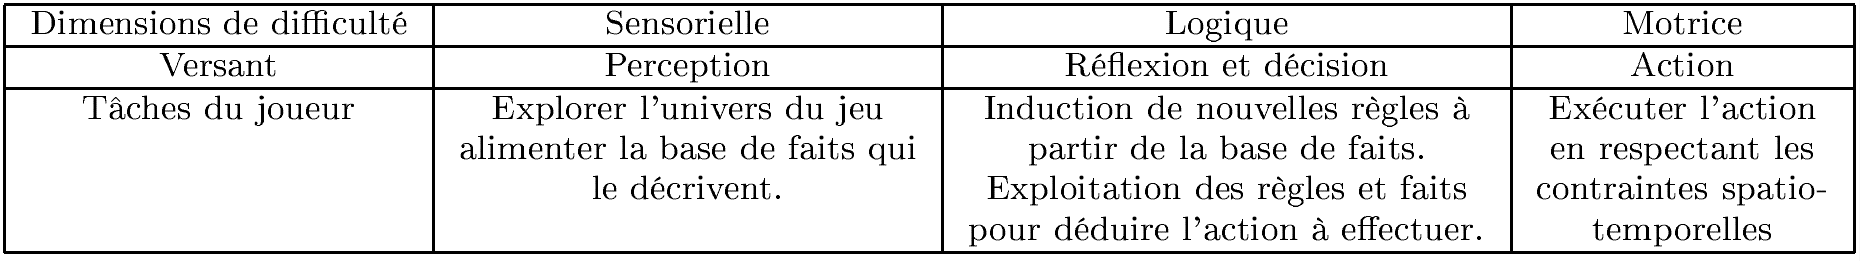
\includegraphics[width=\linewidth]{images/dimensions_difficulte.png}
	\caption{Dimensions de difficulté}
	\label{dimensions_difficulte}
\end{figure}

\paragraph{}Guillaume Levieux [réf] définit donc trois types de difficultés dans le jeu vidéo :
	\begin{itemize}
		\item la difficulté sensorielle : décrit l’effort que doit fournir le joueur pour obtenir de nouvelles informations sur l’état de l’univers du jeu. Ces informations nouvelles correspondent à toute information que le joueur ne peut pas déduire des faits et règles logiques qu’il connaît déjà.
		\item la difficulté logique : décrit l’effort que doit fournir le joueur pour exploiter les informations dont il dispose, c’est à dire comprendre le fonctionnement de l’univers par induction, et choisir la prochaine action à réaliser par déduction.
		\item la difficulté motrice : décrit le niveau de précision spatiale et temporelle dont le joueur doit faire preuve lorsqu’il exécute une action.
\end{itemize}
A titre d’exemple, on peut associer un type de jeu par type de difficulté. Les jeux d’aventure se basent essentiellement sur la difficulté sensorielle, les jeux de stratégie sur la difficulté logique, et les jeux d’actions sur la difficulté motrice. Bien sur, chaque jeu est composé de chacune des trois dimensions, mais exploitées dans des proportions différentes.
		
		\paragraph{\emph{Punitivité}\\ \quad}
Il s’agit de différencier la difficulté du jeu de la punition en cas d’échec. Ces punitions peuvent être dans l’ordre de sévérité : le respawn instantané, celui avec délai, la sauvegarde libre, le checkpoint, les vies limitées et la permadeath (mort immédiate et définitive). Ainsi, un jeu peut être très difficile mais peu punitif (\emph{Super Meat Boy}) ou plus facile mais très punitif (\emph{Binding of Isaac}, \emph{Diablo} en mode hardcore). Lorsqu’il est à la fois difficile et punitif, le jeu entre alors dans la catégorie des jeux Hardcore.

		\paragraph{\emph{Le casual et le hardcore}\\ \quad}
Difficulté et punitivité contribuent donc, parmi d’autres facteurs, à créer une relation entre le jeu et le joueur. Plus celles-ci vont être élevées, plus on va s’éloigner du jeu casual pour se rapprocher du jeu hardcore, où un véritable investissement devient nécessaire pour accomplir le jeu. Il nécessite alors un temps d’investissement important ou une concentration soutenue (difficulté), chaque action va peser (punitivité) et demander au joueur de s’investir, à l’inverse du jeu casual.		
		
		\subsubsection{Pourquoi aime-t'on la difficulté?}
			\paragraph{\emph{Chimiquement} \\ \quad}
Le jeu vidéo est capable de fournir aux joueurs des sensations permettant de délivrer au cerveau dopamine ou adrénaline. L’expérimentation du flow state permet aussi au joueur un ressenti qu’il va chercher à renouveler.

			\paragraph{\emph{L’engagement} \\ \quad}
Le jeu vidéo a par ailleurs cette particularité de faire que le joueur va avoir la volonté de recommencer un niveau ou une partie après un échec. Et cette volonté aura tendance à augmenter tant que le joueur n’aura pas atteint son objectif. Cette constatation peut être expliquée par la théorie psychosociale de l’engagement, et plus particulièrement du concept de dépense gâchée. Selon cette théorie, plus on a passé de temps dans une activité, à apprendre quelque chose ou dans une réalisation, moins on est enclin à y renoncer, sous prétexte du temps inutilement passé à s’y consacrer. Dans le jeu “je ne vais pas abandonner après être arrivé aussi loin !”. L’engagement (et l’attachement aux valeurs) est d’autant plus important que l’investissement a été important, que ce soit en terme de temps, d’efforts, de sacrifices, de souffrance, etc.

			\paragraph{\emph{Dissonance cognitive} \\ \quad}
Par ailleurs, l’humain (entre autre) est mal à l’aise et ressent une tension désagréable lorsqu’il est en état de dissonance cognitive. Cette dissonance est ressentie lorsque l’individu est en présence de cognitions (connaissances, croyances ou perceptions de soi ou son environnement) contradictoires ou incompatibles entre elles.
Cet état entraîne un inconfort psychologique, parfois une réaction émotionnelle, qui pousse la personne à penser ou agir. pour rétablir son équilibre cognitif à l’aide de stratégies inconscientes de rationalisation. L’éveil peut prendre bien des formes, la soumission, la rationalisation, la fuite, un comportement ou une action délibérée, la modification de ses croyances, attitudes ou connaissances pour les accorder avec la nouvelle cognition. Dans le jeu vidéo, cela se traduit par une auto justification de la persévérance du joueur, ou un rejet radical de l’activité. On va se trouver des excuses, etc.

			\paragraph{\emph{Découverte et apprentissage}  \\ \quad}
Ces principes sont primordiaux pour un certain nombre de joueurs.  Que ce soit la découverte d’un monde immense, des capacités de son personnage, des mécanismes du jeu ou encore d’un univers particulier, le plaisir réside dans le fait que rien n’est acquis et se découvre à force d’expérimentations et d’échecs. Au fur et à mesure de ses expériences et observations, le joueur va alors suivre une courbe de progression généralement logarithmique très gratifiante qui va l’inciter à poursuivre son apprentissage pour parfaire sa maîtrise du jeu. Cet intérêt est d’ailleurs suffisamment fort pour qu’une certaine communauté de joueurs complète ses connaissances à l’aide de forums, wiki ou vidéos qu’elle aura elle même mis en ligne.

			\paragraph{\emph{Auto-détermination} \\ \quad}
R. Ryan et al propose d’expliquer la motivation du joueur à travers l’auto-détermination. Ils considèrent que les jeux vidéo satisfont des besoins psychologiques et permettent le développement d’un sentiment d’autonomie, de compétence et de connexion. L’autonomie décrit à la fois le fait que l’investissement du joueur est volontaire et que le joueur possède une autonomie au sein du jeu.

			\paragraph{\emph{Auto satisfaction et dépassement de soi} \\ \quad}
Le plus grand plaisir qu’un joueur peut ressentir en jouant à un jeu difficile ou hardcore, est le sentiment d’auto satisfaction lorsqu’il réussit enfin à accomplir son action. A force d’efforts ou d’entraînement, il réussit à réaliser ce qu’il croyait impossible au premier abord, parce qu’il ne comprenait pas comment y arriver ou n’était simplement pas capable de le faire, par manque de techniques, d’imagination ou d’entraînement. Ce dépassement de soi (technique, intellectuel ou physique) est déjà gratifiant en soi, et récompense le long apprentissage auquel s’est adonné le joueur.

C'est la \textcolor{orange}{réussite} d'un challenge \textcolor{orange}{difficile} qui est satisfaisante, et non directement son accomplissement. À l'inverse, une majorité va choisir une difficulté normale plutôt que facile ou difficile, car les gens aiment \textcolor{vert}{faire} quelque chose qui représente un \textcolor{vert}{challenge modéré} : pas le choisir ou le réussir, moins glorieux.

			\paragraph{\emph{L’enjeu} \\ \quad}
C’est aussi un grand pourvoyeur de plaisir. Un fort enjeux va inciter le joueur à ne pas jouer à la légère, à s’impliquer et donc à s’appliquer dans sa partie. On notera que l’enjeu est d’autant plus fort lors de partie multijoueur : les actions d’un joueur peuvent potentiellement influencer l’expérience de jeu de chacun des autres joueurs. En confrontation, il faut arriver à surpasser l’autre joueur, qui va faire de son mieux pour vous en empêcher. En collaboration, où l’erreur de l’un peut alors aussi coûter aux autres. L’enjeu crée alors un sentiment de tension, qui va lui même renforcer l’immersion du joueur.

\paragraph{}Enfin l’intérêt des joueurs pour les jeux difficiles ou réputés comme tels, peut aussi s’expliquer par une certaine \emph{nostalgie}, une forme d’\emph{élitisme} voir de snobisme envers les jeux/joueurs dits casuals, mais surtout aussi par le plaisir ressenti par la réussite d’un défi qui leur est posé. Une forme de frustration idéalement dosée et que l’on a surmontée.

	\subsubsection{Difficulté dans les Serious Games}
Les SG ont la particularité de conjuguer les mécanismes classiques du jeu vidéo à des objectifs sérieux de nature différente. Ces objectifs peuvent être la transmission de connaissances ou de valeurs si la visée est intellectuelle, ou bien un travail sur la forme ou les capacités physiques du joueur. Dès lors, la difficulté du jeu se dote d’une nouvelle composante relative à cet objectif thérapeutique.\\
Dans le cas de SG physiques, qui utilisent des périphériques comme la wii board, la kinect ou le PSmove par exemple, on pourra assimiler cette nouvelle composante à la difficulté motrice déjà définie. A la difficulté de synchronisation oculo-motrice de la main sur le contrôleur, s’ajoute des difficultés physique telles que la précision, l’endurance, l’équilibre ou la souplesse.
Dans les jeux dont l’aspect sérieux est intellectuel, l’objectif sérieux peut venir enrichir la difficulté logique du jeu (difficulté de compréhension, de raisonnement, de mémoire).
Dans les jeux sérieux dont le but est une rééducation psychomotrice, il est aussi important d’envisager un nouvel aspect de difficulté de type émotionnel. Il faut en effet prendre en compte l’enjeu médical et la possible fragilité du joueur, dont la progression ou non peut avoir un impact important sur son mental.
\newpage
		
\subsubsection{\emph{Encart proposition \\} Proposition d'une nouvelle composante : la difficulté émotionnelle}
Nous avons vu dans notre recherche documentaire que sont définies trois types de difficultés dans les jeux vidéo. [Levieux, 2011]\cite{Levi11} définit ainsi la difficulté sensorielle, la difficulté logique et la difficulté motrice.

\paragraph{}Il est aussi possible d’envisager une dimension émotionnelle dans la difficulté. Cette difficulté peut se manifester lors de la réalisation d’une action dont la réussite ou non est importante pour le joueur, lors d’une confrontation avec une situation, un problème ou un objet dont le joueur a peur ou le rend particulièrement mal à l’aise par exemple : mise en situation d’une phobie, d’une scène en désaccord avec ses moeurs ou convictions, lui rappelant des évènements difficiles ou traumatisants, etc.
 \paragraph{}
On peut citer l’exemple du jeu \emph{Paper Please}, dans lequel on incarne un employé travaillant à un poste de frontière et qui contrôle l’accès au pays. Dans ce jeu, le joueur sera partagé entre respecter les consignes strictes d’immigration et le caractère émotionnel et personnel des personnes souhaitant entrer dans le territoire avec des histoires et des motivations personnelles, personnes pour lesquelles il nous faudra décider si on autorise ou on restreint l’accès. Cette décision pourra être particulièrement difficile car elle se fera au risque de perdre son emploi et ne plus pouvoir faire survivre sa famille ou d’être en profond désaccord, voir en situation de dégoût, avec soi-même...\paragraph{}
Le joueur peut aussi s’imposer lui-même un certain nombre de contraintes, pour être en accord avec ses principes. Ces contraintes peuvent être d’ordre moral ou éthique (refus de tuer un personnage dans le jeu ou d’effectuer une mauvaise action), ou plus artificiel comme vouloir jouer de manière “Role Play” et donc s’interdire certaines actions ou au contraire s’en imposer d’autres. Ainsi, même si le joueur sait qu’il gagnerait à réaliser une action particulière et qu’il est en mesure d’y parvenir, il ne passera pas nécessairement à l’œuvre. 
\paragraph{}On pourra ainsi citer l’exemple du jeu \emph{Valkyrie Profile}, dans lequel le joueur peut contrôler un personnage principal, ainsi qu’un groupe de personnages secondaires. Durant les phases de combats tactiques, le joueur a la possibilité de sacrifier un personnage secondaire afin d’obtenir une puissance phénoménale, qui se révélera souvent nécessaire d’acquérir tant la difficulté du jeu est élevée. Mais ces sacrifices sont permanents et l’avatar, ainsi que le joueur, devront les assumer et vivre avec la conscience d’avoir tuer ces personnages, ce qui fera évoluer différemment l’histoire.
\paragraph{}
Un autre aspect émotionnel se trouve dans l’acceptation du déroulement du jeu. Dans un jeu multijoueur compétitif ou opposant une IA, si l’adversaire emploie une stratégie ou une technique particulièrement frustrante pour le joueur, celui-ci peut s’en trouver affecté (colère, énervement, mauvaise estime de soi, mauvaise foi). Si cette situation continue ou est répétée, ou bien que malgré une difficulté modérée notre joueur continue de perdre ou de se faire mener en bateau pour une raison ou une autre, la difficulté émotionnelle deviendra telle qu’il pourra préférer abandonner. Cette situation particulièrement fréquente dans les jeux multijoueur en ligne peut mener à ce que l’on appelle couramment un \emph{rage quit}, qui désigne familièrement le fait pour un joueur de quitter une partie en cours sous l'effet de la colère.

\paragraph{}On peut noter que cette difficulté peut en fait impacter directement les trois autres aspects de la difficulté précédemment cités. Un joueur qui aura réellement peur perdra de ses capacités sensorielles, logiques ou motrices par exemple. Cet impact n’est cependant pas systématique : une situation obligeant le joueur à réaliser une action allant à l’encontre de ses principes n’affectera pas ses capacités, mais le joueur hésitera cependant à réaliser l’action qu’il sait nécessaire ; il aura compris la situation, trouvé la solution à sa réalisation et est physiquement capable de la réaliser, mais ne souhaitant pas la faire, différera son exécution, voir l’évitera si possible.

\paragraph{}Dans le cas particulier d’un Serious Game pour la réhabilitation motrice, la difficulté émotionnelle peut se situer dans l’intérêt particulier qu’a le joueur-patient dans l’évolution de sa pathologie. Il est nécessaire en phase de rééducation que le patient soit capable de sentir qu’il progresse afin de garder sa motivation et poursuive son travail. Une confrontation trop fréquente à des gestes qu’il n’est pas encore/toujours pas capable de réaliser parce que trop difficile, aura pour conséquence de lui rappeler sa déficience et pourra lui faire perdre toute ambition thérapeutique.

\paragraph{}Cette dernière constatation pose la question de savoir si la difficulté d'un jeu vidéo classique est comparable à celle d'un jeu thérapeutique.\\ Le serious game thérapeutique se pose dans un contexte précis, dans lequel les joueurs sont des personnes blessées, physiquement et/ou psychologiquement. Il est ainsi difficile de s'attendre de leur part à des réactions classiques et c'est un facteur dont je pense qu'il est important de tenir compte. Bien doser l'évolution de la difficulté ou des exigences faites envers le joueur est ainsi primordial pour s'assurer du maintien de l'activité, et donc de l'amélioration de son état. Si le joueur se sent biaisé par l'application, à cause d'une difficulté trop importante ou d'une évolution trop rapide, il aura tôt fait de cesser de jouer et le jeu, aussi efficace puisse t-il être par ailleurs, n'aura alors aucun impact.
		
	\subsubsection*{Relation entre les différents paramètres d'un jeu vidéo}
Afin de mieux comprendre pourquoi le jeu vidéo est un média apprécié et comment ses différents paramètres peuvent être utilisés pour des objectifs sérieux, j'ai cherché à trouver le lien entre ces composantes. Dans un contexte de rééducation, on va aussi chercher à connaître quelles théories sont intéressantes pour les thérapeutes, pour qu'ils puissent réaliser un classement par importance pour la thérapie. Comprendre les relations qui existent entre le jeu vidéo et le joueur pourrait aussi permettre de mieux comprendre les mécanismes en jeu et mieux orienter les exercices d'éducation ou de réhabilitation.
\begin{figure}[htbp]
Schéma inspiré des théories comportementales et psychologiques et de concepts mis en place dans les jeux vidéo.
	\centering
	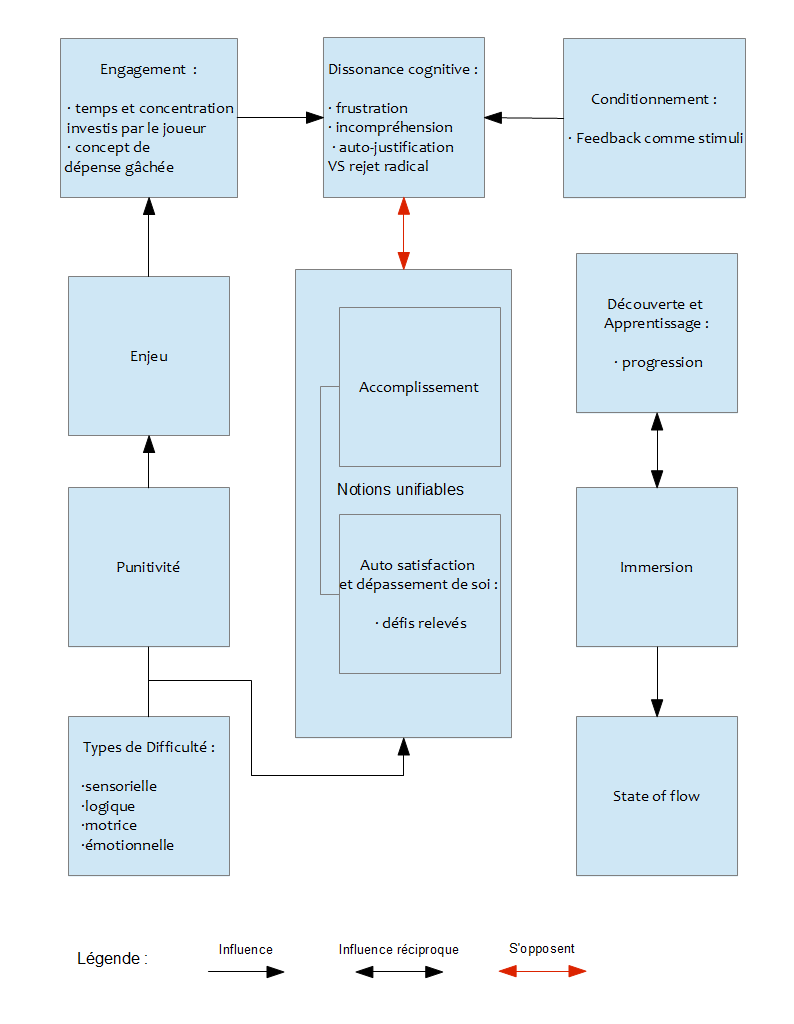
\includegraphics[height=19.6cm]{images/lien_theories}
	\caption{Relation entre les principaux ressorts psychologiques d'un jeu vidéo}
	\label{lien_theories}
\end{figure}			



%****************** Subsection 4 : Réhabilitation
		\subsection{Réhabilitation}
Un autre aspect est la dimension médicale de la rééducation. Connaître les enjeux, les contraintes, le contexte médico-social d'une réhabilitation ainsi que les techniques existantes s'avérait donc nécessaire. Cette partie est la synthèse de mes entretiens et investigations dans ce domaine qui ne m'était encore que peu connu.

		\subsubsection{Contexte socio-médical : connaître l'AVC}
L'accident vasculaire cérébral, ou AVC, parfois aussi appelé attaque cérébrale, est un déficit neurologique soudain d'origine vasculaire causé par un infarctus ou une hémorragie au niveau du cerveau. Les symptômes peuvent être très variés d'un cas à l'autre selon la nature de l'AVC ou l'endroit et la taille de la lésion cérébrale, ce qui explique un large spectre : aucun signe remarquable, perte de la motricité, perte de la sensibilité, trouble du langage, perte de la vue, perte de connaissance, décès, etc.	

		\paragraph{\emph{L’accident vasculaire cérébral (AVC) est un événement de santé fréquent}\\}
Dans les pays occidentaux, près d'un individu sur 600 est victime d'un AVC chaque année, soit près de 120 000 accidents par an en France. L'AVC est une cause fréquente d'hémiplégie chez les victimes et reste une des principales causes d'invalidité. \\
La récupération des fonctions motrices, de la parole ou de la compréhension dépendent pour beaucoup de l'âge du patient et de son atteinte au niveau du cerveau.

\paragraph{•}L’âge moyen de survenue d’un AVC est de 73 ans : 70 ans pour les hommes et 76 ans pour les femmes.

\paragraph{•}   Les données préoccupantes concernant l’augmentation des AVC dans la population des moins de 65 ans concernent plus les femmes (+ 12,9\%) que les hommes (+9,7\%). Ce phénomène épidémiologique préoccupant est à examiner dans un contexte de diminution de l’espérance de vie en bonne santé (sans incapacité) qui est passée de 62,7 ans à 61,9 ans pour les hommes et de 64,6 ans à 63,5 ans pour les femmes, en seulement deux ans (entre 2008 et 2010)

\paragraph{\emph{L’accident vasculaire cérébral (AVC) est un événement de santé grave}\\}

	\paragraph{En termes de mortalité :}
    L’AVC représente la troisième cause de mortalité pour les hommes (après les cancers « de la plèvre, de la trachée, du larynx ou des poumons » et les cardiopathies ischémiques) et la première pour les femmes avant le cancer du sein.\newline
    En 2008, l’AVC a été responsable de 33 000 décès.

	\paragraph{En termes de handicap :}
Dans les pays occidentaux, l’accident vasculaire cérébral est une cause majeure de handicap acquis de l’adulte, la deuxième cause de démence après la maladie d’Alzheimer et la troisième cause de mortalité.	\newline

    L’AVC est souvent responsable de séquelles qui affectent la qualité de vie des patients. 

 \paragraph{•}
Les atteintes peuvent être motrices, sensitives, sensorielles et cognitives (avec notamment des troubles de la mémoire) 

\paragraph{•}Un mois après l’AVC, pour les personnes ayant survécues, les dépressions sont fréquentes et il est à noter que seulement 41\% d’entre elles n’ont plus de symptômes, ainsi~:
\begin{itemize}
	\item 25\% présentent un handicap léger ou modéré
	\item 34\% ne peuvent marcher sans assistance.
\end{itemize}
 
		\paragraph{L'AVC et Hammer \& Planks\\}
Hammer \& Planks est né d'un projet d'une étudiante en ergothérapie dont le but était de proposer un jeu servant à travailler l'équilibre chez des personnes hémiplégiques ayant été victimes d'un AVC. Aujourd'hui, H\&P peut être utilisé aussi bien pour travailler son équilibre, ses membres supérieurs son tronc ou sa capacité d'attention.   	
	\paragraph{}
Lors de mes six mois de stage, j'ai ainsi été en relation avec plusieurs docteurs en médecine, des kinésithérapeutes ainsi que des ergothérapeutes.

	\subsubsection{Enjeux et objectifs thérapeutiques de la réhabilitation} \label{objectifs_therapeutiques}
Le principe de base est de faire un bilan initial.  A partir de ce dernier on dégage des objectifs  de rééducation. Pour atteindre ces objectifs, il existe des moyens de rééducation (exercices, physiothérapie, jeux vidéos, etc.) qu'il faut adapter au patient.

\paragraph{Les grand axes de rééducation}
\begin{itemize} 
	\item Récupérer la commande motrice 
	\item Diminuer la douleur
	\item Assouplir les muscles 
	\item Récupérer la sensibilité 
	\item Renforcement musculaire 
	\item Transfert du poids du corps 
	\item Travail de l'équilibre bipodal / unipodal 
	\item Travail du schéma de marche
\end{itemize}

	\textbf{\emph{Définitions}\\}
• \emph{La spasticité} consiste en un étirement rapide d'un muscle qui entraîne trop facilement sa contraction réflexe qui dure un certain temps. \\
• \emph{L’hypertonie spastique} (musculaire) est une contraction réflexe du muscle qui s'oppose à l'étirement.\\

	\textbf{\emph{Signifiant VS significatif}\\}
L’aspect signifiant/significatif est un terme utilisé en ergothérapie pour définir le sens qu'a une activité auprès d’un patient.\\
• Une activité peut être qualifiée de \emph{\textcolor{orange}{significative}} quand elle revêt un \textcolor{orange}{sens social commun}. Par exemple dans notre cadre, les jeux vidéo et notamment la Wii, peuvent être significatifs pour les personne âgées de 10 à 30 ans, car ils sont beaucoup utilisés dans cette tranche d'âge.\\
• Une activité est dite \emph{\textcolor{vert}{signifiante}} quand elle a du sens pour la personne de \textcolor{vert}{manière personnelle}. Par exemple, faire la vaisselle est \textcolor{orange}{significatif }car on \textcolor{orange}{doit} la faire. Mais en général les personnes n’aiment pas la faire et elle est donc pour eux non signifiante. Alors que ‘moi’, c'est une activité que ‘j’’apprécie :  elle a donc pour ‘moi’ un sens motivationnel et est alors signifiante.

	\paragraph{\emph{Cas de l’hémiplégie} \\}
C’est une pathologie qui n’est pas évolutive, on ne peut que récupérer. Cette récupération est différente chez tous les patients, en fonction de leur âge, leur condition physique, de la gravité de la pathologie et de la rééducation mise en place.

	\subsubsection{Cas de l'hémiplégie}
\paragraph{\emph{Mouvements analytiques / Motricité fine} \\ }
Les hémiplégiques vont présenter des troubles de la sensibilité et des troubles de la commande volontaire. Un problème nerveux peut entraîner une augmentation du tonus musculaire pouvant provoquer une spasticité ou une hypertonie. 

\paragraph{}
Parmi les objectifs, on va donc tout d’abord chercher à récupérer une commande motrice normale, puis à rééquilibrer les capacités (musculaires et nerveuses) et enfin renforcer les capacités musculaires. Dans la pratique, le patient va donc tout d’abord chercher à retrouver un mouvement précis, puis à être capable de l’effectuer de manière fluide et plus rapide, puis à pouvoir mettre de la force dans son geste, pour vaincre la gravité ou supporter un poids/une résistance par exemple.

\paragraph{}
Pour ‘vaincre’ la spasticité du patient, le praticien doit pratiquer des manipulations sur le patient pour étirer ses muscles. Il est donc difficilement envisageable de gamifier cet aspect de la rééducation.\newline
Déficit léger : travail en 3D possible     \quad$ \rightarrow $\quad       Épaules\\
Déficit lourd : travail en 2D uniquement  \quad $\rightarrow $\quad      Poignets et mains

	\paragraph{Paramètres\\}
Récupération de la commande volontaire, amplitude articulaire, spasticité, phase aiguë VS phase chronique( $ \rightarrow $ spastique)\\
Plasticité cérébrale : intensive et ciblée. \newline

Les thérapeutes veulent~: 
\begin{itemize}
	\item des mouvements répétitifs fins
	\item un type précis de mouvement (rotation par exemple)
	\item pouvoir paramétrer les exercices
	\item lâcher / écarter (voir le système PABLO)
\end{itemize}

	\paragraph{\emph{Sensibilité} \\ \quad}
Exercice : le patient ferme les yeux, le thérapeute lui donne un petit objet dans la main. Que ressent-il? Quelle texture, quelle forme? \\
En fait, on lui présente avant l’exercice une série d’objets (éponges de différentes tailles et souplesses, figurines en bois de différentes formes). Puis, yeux fermés, il doit essayer de reconnaître l’objet que lui présente le thérapeute en identifiant ses propriétés haptiques et tactiles.
\paragraph{} 
Ce travail de la sensibilité est particulièrement important pour les mains, riches en capteurs tactiles. Il est par ailleurs nécessaires de travailler cet aspect pour que le cerveau “n’oublie pas” en réutilisant les connexions neuronales spécifiques. Par ailleurs, on peut aussi travailler la sensibilité d’autres membres comme les pieds, ce qui est particulièrement important notamment dans le cadre de la marche où la perception des aspérités/irrégularités du sol est importante.\\
Cet aspect de la rééducation est complémentaire de celui de la récupération de la préhension. Le patient aura ainsi la capacité (commande, force) de tenir un objet, mais le lâchera faute d’informations sensorielles suffisantes.

	\paragraph{\emph{Équilibre} \\ }
Équilibre assis d’abord si la personne n’est pas capable de se tenir debout. Si son équilibre est vraiment précaire, il peut être nécessaire de placer le patient au milieu d’un cercle de maintien, ou de surveiller la personne.\\
On peut ensuite passer à un travail de l’équilibre debout, en diminuant progressivement l’écart entre les deux pieds. Un autre facteur de difficulté va être de fermer les yeux, le patient doit être capable de maintenir son équilibre.

	\paragraph{\emph{Diminuer la douleur} \\ }
Pour cela, plusieurs moyens. On peut prescrire des traitements : au niveau neurologique, articulaire ou musculaire ; de la physiothérapie ou une mobilisation passive (manipulation kiné). Mais pas de jeux.
Pour les lombalgiques : en cas de crise aiguë, du repos, puis rapidement refaire de l’exercice.
En phase chronique, augmentation du tonus musculaire et renforcement musculaire.

	\paragraph{\emph{Transfert de poids} \\ }
Chez les hémiplégiques gauche, le centre de pression va se situer à droite. On va donc chercher à déplacer le centre de pression du patient vers la gauche jusqu’à atteindre le milieu du corps, car il a la force et la commande. Voir équilibre.

	\paragraph{\emph{Renforcement musculaire} \\ }
A première vue, peu adapté à l’hémiplégie, on visera plutôt à retrouver un mouvement, une commande motrice (ou alors en fin de rééducation).

	\paragraph{Paramètres \\}
Fréquence, amplitude, durée du maintien, nombre de mouvements réalisés / répétitions, vitesse, fluidité.

\paragraph{}En phase finale de récupération : endurance, périmètre de marche, performance : vitesse (de marche), marche sur terrain plat ou accidenté, contrôle moteur, coordination, travail dans les escaliers, relevé du sol (fonctionnel), retournement et transfert (passage du lit à assis, de assis à debout et inversement).

	\subsubsection{La réhabilitation au quotidien}
Dans le cadre de mon travail sur le projet Hammer \& Planks, j'ai réalisé plusieurs séances d'observations de séances de rééducations chez des kinésithérapeutes. Afin de mieux cibler les attentes et besoins à la fois des thérapeutes et des patients, il me semblait primordial d'assister directement à ces étapes de la réhabilitation. Je souhaite ici partager mon expérience au travers le compte rendu d'une demie journée d'observation chez le kinésithérapeute Didier Costeau, exerçant à Montpellier. Ce résumé est important en ce qu'il permet de saisir les enjeux sociaux, médicaux et techniques de la réhabilitation. M. Costeau a ça de particulier qu'il utilise dans son métier des jeux vidéo classiques dont il dérive l'utilisation dans un but thérapeutique.

	\subsubsection*{Organisation}
Une grande salle remplie de machines, dans laquelle les patients viennent en groupe tout au long de la journée. Les patients sont majoritairement hémiplégiques ou tétraplégiques, et se déplacent pour beaucoup en fauteuil.

\paragraph{}
D. Costeau passe d'un patient à un autre pour les préparer sur la banquette ou sur une des machines à sa disposition. Il dispose entre autre d'appareils de musculation (traction, pectoraux, etc), de vélos, d'un stepper ou d'un Huber (machine permettant de faire travailler l'équilibre, 80 muscles du corps), ainsi que d'un Segway. Il les aide donc à se positionner sur la machine et éventuellement à la régler (poids, attaches).\\
Puis, selon les exercices à réaliser, M. Costeau propose de réaliser cet exercice à l'aide d'un jeu vidéo en utilisant des consoles et accessoires de la Wii. En attachant une wiimote sur le stepper ou un vélo, le patient va être capable de profiter de l'environnement ludique du jeu vidéo tout en faisant ses exercices de rééducation. Les patients peuvent aussi jouer à plusieurs avec le jeu de tennis de Wii Sport, en tenant directement la wiimote dans leur main.\\
Par ailleurs, il utilise aussi la balance de la wii board, en ayant mis en place un système permettant de poser une planche sur la board, afin qu'une personne en fauteuil puisse y monter et l'utiliser. Cela permet de travailler l'équilibre ou la force des jambes d'un patient. Une variante propose même 2 bâtons de ski, afin qu'une personne ne pouvant pas beaucoup se pencher puisse s'aider des bâtons et s'appuyer dessus. Dernière variante, accrocher une wiimote au dessus d'un casque, système notamment utilisé pour les personnes présentant une déficience motrice cérébrale, pour leur faire travailler leur port de tête.\\
A chaque fois, l'idée est évidemment de proposer un jeu afin d'offrir un feedback, ludique qui plus est, un suivi des progrès et une ambiance décontractée.

\paragraph{}Autre fait notable, de nombreuses cordes de tension traversent la pièce ; elles ont été installées afin de pouvoir garder le dos des patients cambré. En effet, le dos a besoin d'être cambré, mais la colonne a tendance à se tasser à force de rester assis; fait malheureusement inévitable chez les personnes en fauteuil.

\paragraph{}Dans les pratiques plus classiques, j'ai pu assister à des manipulations directes du praticien sur les patients (travail sur les membres inférieurs ou supérieurs : extensions, flexions, jeu de force) ou à l'aide au réapprentissage de la marche, en mettant un patient debout et en le maintenant tout au long d'une marche.

	\subsubsection*{Remarques, ressentis (mots clefs) }
		\paragraph{\emph{Aspect Social – Jouer ensemble}\\}
Première impression en arrivant : les séances se déroulent en groupe, et tout le monde \textbf{communique} !
Les gens se parlent, blaguent, jouent ensemble si c'est possible, etc. \\
C'est une constatation évidente, et cela m'a été confirmé oralement après, les patients préfèrent être en groupe : "On ne viendrait pas sinon". En arrivant, une personne jouait au tennis avec la Wii, et dès son arrivée, une patiente a voulu la rejoindre pour partager une partie multijoueur. Malgré la différence de niveau, tout le monde y trouvait du plaisir et y mettait du sien. Même les non joueurs se sentaient impliqués et commentaient la scène. \\
A mon avis, c'est un élément très important à prendre en compte. Il faut tout de même penser à intégrer le fait que les patients n'ont ni le même handicap, ni a priori le même niveau de joueur dans un jeu particulier.

\paragraph{}Une suggestion qui tient à cœur le kiné, car très importante, serait la possibilité de jouer à plusieurs même à des endroits différents. Par exemple deux patients dans des chambres différentes, mais qui pourraient tout de même jouer une partie ensemble.

		\paragraph{\emph{Les Jeux : gamification de la thérapie}\\}
De manière générale, les patients, l'âge ayant l'air d'un critère peu discriminant, ont clairement adopté l'usage des jeux vidéo pour leur séance de kiné. De la jeune fille ou jeune adulte, au monsieur de près de 80ans, les patients jouent, et aiment ça. C'est à la fois surprenant et non. Si les dernières générations ont toujours connu les divertissements numériques, ce n'est pas le cas de la plupart des patients qui viennent au cabinet. Bien que peu voir pas à l'aise avec la technologie, ils reconnaissent aisément que cela peut être divertissant et se prêtent vite au jeu de la comparaison des résultats par exemple.
\begin{quotation}
Ex : un patient de 78 ans (militaire, strict, sportif), qui "ne connaît pas Facebook, Google, Twitter et iPad, n'a pas d'ordinateur et n'en veut pas", apprécie les jeux et la console, car "Ça vous gnaque ! J'ai fait 8km, à mon âge !" après une séance de stepper avec la Wii.    
\end{quotation}
Au niveau des performances, on peut citer un autre exemple, d'un patient utilisant un vélo équipé d'une Wiimote (cf partie feedback) : en l'observant, j'ai pu remarqué qu'il avait réalisé la majorité du temps de course les yeux fermés, comme pour se concentrer. Cependant, sur les 5 dernières minutes des 30, il a réouvert les yeux et j'ai pu constater que son allure augmentait alors significativement (de l'ordre de 30\%). On peut supposer que le feedback donné par le jeu n'était pas complètement étranger à cette différence (bien que probablement pas le seul facteur).    
Une autre patiente utilisant la wii balance board avec son fauteuil pour jouer au snowboard, m'a confié que cela la lui permet de travailler aussi bien, avec une fatigue équivalente, mais que c'est « plus sympa »(bien que répétitif aussi à la longue) et « donne un objectif » (celui du jeu).

\paragraph{}Pour nuancer ces propos, tous les patients n'ont cependant pas joué pendant leur séance ce jour là. Un monsieur dont l'hémiplégie était importante m'a expliqué qu'il ne pouvait pas jouer, aucun jeu ne pouvant s'adapter à ses capacités motrices réduites, malgré les nombreux arrangements qu'a réalisés Didier Costeau. Pour d'autres, ce n'était tout simplement pas prévu/possible de part la nature des exercices qu'ils devaient réaliser. Enfin, au moins une personne ne semblait pas du tout intéressée, mais je n'ai pas réussi à en connaître la raison .

		\paragraph{\emph{Diversité – Variété}\\}
C'est LE problème décrit par tous les patients et le kiné : le manque flagrant de diversité, de représentations. Diversité des jeux, des niveaux, des bonus, de musiques (tout le monde se plaint !), d'obstacles, d'exercices, de la difficulté, etc.

		\paragraph{\emph{Cohérence - Adaptation}\\}
Autre problème actuellement, parfois un problème de cohérence entre les gestes / mouvements du patient et le feedback du jeu. Notamment pour l'instant, un vélo customisé pour pouvoir être utilisé par une personne dans un fauteuil, vélo auquel on rajoute deux bras elliptiques sur lesquels on accroche une wiimote. La wiimote effectue donc des mouvements verticaux, et actuellement, le jeu associé est un jeu de course à pied. Malheureusement, la vitesse de mouvement de la wiimote fait que l'avatar du patient court extrêmement lentement, sans cohérence avec sa performance à vélo.
Il faut donc diversifier l'offre pour s'adapter au besoin, en proposant gameplay et feedback cohérents. Avoir une solution de jeu pour chaque type de mouvements / exercices que l'on souhaite faire. Cela passe par l'utilisation d'un panel de périphériques plus large.

\paragraph{}Dans le même domaine, un problème reste le temps passé par le soignant à configurer les jeux, matériels et parties. Normalement, la configuration matérielle se fait une fois pour toute (lors de ma séance d'observation, il a fallu le refaire suite au changement de la console), mais c'est un point à penser pour éviter de faire perdre du temps dans le cas ou cela doit se reproduire.
Certains patients sont capables de choisir et lancer eux même leur jeu ainsi qu'une partie, mais ce n'est pas le cas de tous, et le soignant doit alors intervenir régulièrement. La navigation dans les menus est difficile. Il faudrait imaginer un système permettant de s'affranchir de cette aide, notamment si on entre dans l'hypothèse où les patients jouent chez eux sans personne alentours pour les aider (ou dans une optique de recherche d'autonomie). Cela peut cependant se révéler difficile pour les patients les plus atteints (capacités motrices extrêmement limitées, locution fortement diminuée). Cette remarque est d'autant plus importante qu'un certain nombre de patients ont acheté chez eux la Wii (c'est quelque chose à vérifier sur une échelle plus importante) afin de pouvoir s'entraîner chez eux.

\paragraph{}Le soignant veut aussi pouvoir adapter facilement la difficulté d'un exercice en fonction du patient. Avec les appareils de musculation, il peut par exemple changer la valeur de poids à soulever ou la tension exercée, et l'adapte pour chaque patient.
Dans ce genre là, s'inspirer du système de HUBER, qui offre un suivi des résultats pour chaque patient.

	\subsubsection*{Aspect Médical}

		\paragraph{\emph{Lien avec la vision}\\}
Vu aussi lors de mes recherches documentaires, le lien étroit entre la vision et les capacités motrices. J'ai donc voulu confirmer cette hypothèse auprès des patients et du kiné. Celui-ci m'a alors parlé du problème de plasticité cérébrale. Brièvement, cela représente l'aspect déformable du cerveau et sa capacité à modifier l'organisation de ses réseaux de neurones en fonction des expériences vécues par l'organisme. 

En plus d'avoir sa vision affectée par son AVC et l'hémiplégie, le patient va avoir tendance à délaisser son coté diminué, que ce soit physiquement ou visuellement. Il est donc important de faire travailler simultanément sa vue périphérique du coté atteint en même temps que les membres affectés, dans le but de recréer des connections neuronales pour re-développer sa vision.

		\paragraph{\emph{Importance des exercices sous-progressifs}\\}
Ce sont des exercices qui décomposent les mouvements et font travailler individuellement ces sous mouvements.

		\paragraph{\emph{Travail bilatéral}\\}
Toujours d'après les recherches dans le domaine, penser à l'importance d'un travail bilatéral dans la rééducation. Voir section \ref{bilateral}


		\paragraph{\emph{Shemes de diagonale}\\}
Les schemes de diagonale représentent le fait que la plupart des gestes que nous faisons (bras et jambes) se font sur un modèle de diagonale (car plus naturelle) dans la mesure du possible. Attraper un objet devant soi ou en hauteur (on croise le bras pour être bras tendu), la marche, le ski ou le snowboard, l'escalade, le tennis, etc.	
	

	
	\subsubsection*{Récupération de lombalgie}
Si la réhabilitation post AVC a été au cœur de mon travail et de celui de NaturalPad, son objectif est de pouvoir proposer ou accéder à des solutions pour divers types de pathologies. Ainsi, un projet de NaturalPad pour lequel j'ai participé à la phase de conception a pour objectif de créer un serious game pour la rééducation de personnes lombalgiques.
\paragraph{}
La lombalgie est un état douloureux du rachis lombaire qui peut être aiguë ou chronique. Les lombalgies affectent une forte proportion de personnes puisque entre 40 et 70\% de la population est touchée à un moment ou un autre. Sous l'effet de la douleur, une majorité des patients va cesser toute activité physique voir même professionnelle. Une de ses conséquences est aussi une démotivation de la personne pouvant aller jusqu'à un état de dépression, notamment dû à l'inactivité et la douleur. Comme préconisé dans le Guide du Dos\cite{backbook}, la reprise et le maintien d'une activité physique sont primordiaux dans le processus de récupération. \\
Le projet de NaturalPad est une application de coaching sportif adaptée à ce besoin et proposant un certain nombre d'exercices physiques gamifiés afin d'encourager la reprise d'activité des utilisateurs.

%****************** Subsection 5 : Système de recommandation
		\subsection{Système de recommandation}	 \label{recommandation}
Les systèmes de recommandation représentent les préférences de l'utilisateur dans le but de proposer des articles à acheter ou à examiner notamment. Dans notre problématique, un système de recommandation pourrait servir à sélectionner les paramètres de jeux, voir le jeu lui même, qui correspondraient le mieux aux besoins du joueur. Rappelons que ces besoins peuvent être soit explicites, notamment à travers les recommandations et exigences du thérapeute, soit plus inconscients. Ces besoins inconscients représentent pas exemple les préférences du joueur-patient en terme de gameplay. Un jeu plus distrayant et motivant pour le patient renforcera son implication dans le programme de réhabilitation, et donc son rétablissement. Pour cela il faut donc à la fois connaître les préférences du patient, explicites ou `découvertes'  grâce à un système d'apprentissage par exemple, mais aussi s'appuyer sur un certain nombre de théories et connaissances que l'on sait efficaces pour renforcer cette immersion. 	
	 
 \paragraph{}
 La proposition est ici de s'inspirer du monde la musique (ou des livres, des films, ou encore des ventes en ligne) et de son système de recommandation.\\
 On pense rapidement à deux types de recommandations. La recommandation sociale, qui consiste par exemple à conseiller à un utilisateur des musiques qu'apprécient des personnes de son réseau, surtout si elles écoutent généralement des musiques identiques. Un autre exemple sur les sites de vente en ligne, où l'on propose à un utilisateur venant d'acheter un objet, une liste de produits ayant été achetés en même temps par d'autres utilisateurs. \\
Le second type de recommandation se base pas non pas sur l'environnement social de l'utilisateur, mais sur le contenu même des objets recommandés. L'idée est alors de chercher à décrire un objet selon certaines caractéristiques, et à faire de même pour les préférences de l'utilisateur. On va ensuite lui conseiller les objets qui semblent être le plus proche des attentes de l'utilisateur en se basant sur ces critères de préférences. 
 
\paragraph{}
Pour Vincent Castaignet, fondateur et directeur de la publication de Musicovery, au-delà de la recommandation éditoriale, il y a différentes manières de proposer des artistes/titres par similarité~:
\begin{enumerate}
	\item d’après les formes musicales sur lesquelles le goût des auditeurs est fondé.
	\item d’après les repères mentaux utilisés par les auditeurs (genres, sous-genres, style).
	\item social  : si tu es membre de cette tribu et aimes cet artiste, alors tu vas aimer ces artistes.
	\item contextuel  : ceux qui écoutent ce titre dans ce contexte écoutent aussi ces titres.
\end{enumerate}
Les passionnés de musique qui cherchent activement préféreront de la similarité type (2), le grand public plus passif de la similarité type (4). Un moteur de similarité intelligent devrait pouvoir combiner ces différentes formes et s’adapter en fonction du profil de chacun.
Pandora est principalement construit sur (1), last.fm est (2) et (3), Musicovery (4). Deezer avec ces 30 millions de playlists a un actif considérable à exploiter en (3) et (4).

 		\subsubsection*{Les différents types de recommandation}
Plusieurs techniques de recommandation ont été proposées : basées sur le contenu, sur des connaissances ou encore des techniques dîtes collaboratives ou sociales. Pour de meilleurs résultats, certaines de ces techniques peuvent être utilisées conjointement dans des systèmes de recommandation hybrides.

	\paragraph{\emph{Propriétés des systèmes de recommandation} \\ \quad}
Les systèmes de recommandation possèdent :
\begin{itemize}
	\item des données de base : données que le système possède avant même de commencer la recommandation
	\item des données d’entrée : données que l’utilisateur fournit au système dans le but que ce dernier lui fournissent des recommandations.
	\item un algorithme qui utilise ces données de base et d’entrée pour générer les résultats.
\end{itemize}

	\paragraph{}
\begin{figure}[hbtp]
	\centering
	On peut distinguer 5 types de systèmes de recommandation
	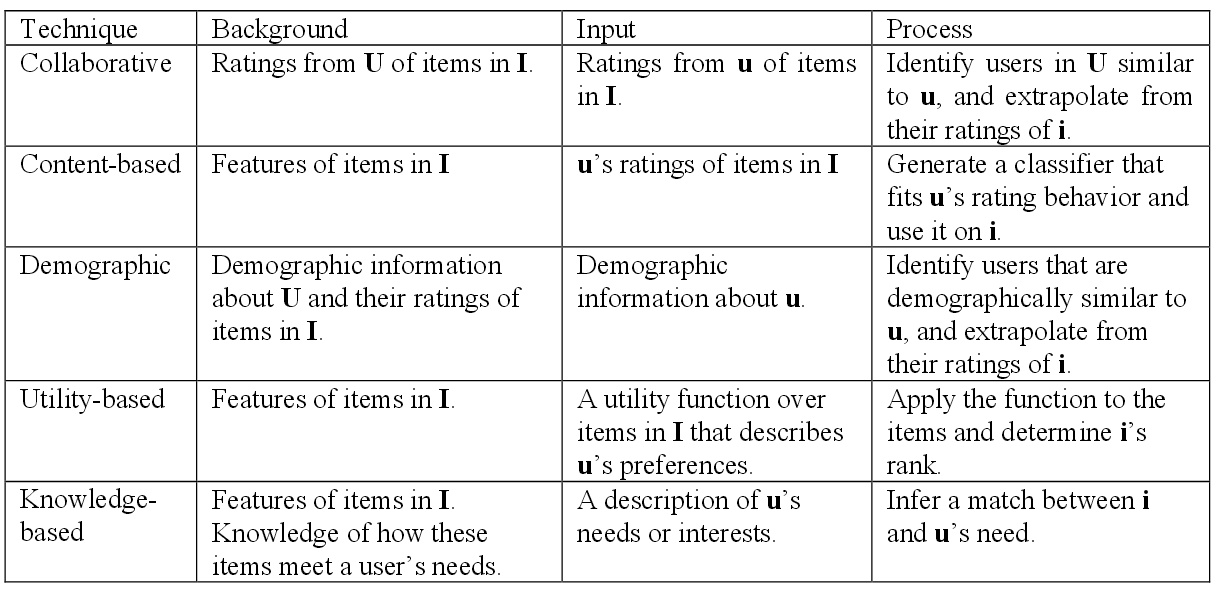
\includegraphics[width=1\linewidth]{images/types_recommandation.png}
	\caption{Techniques de recommandations [R. Burke, 2002] \cite{Burk02} }
	\label{types_recommandation}
\end{figure}    
avec :
\begin{itemize}
	\item I : ensemble d’objets sur lequel sont faites les recommandations
	\item U : l’ensemble d’utilisateurs dont les préférences sont connues
	\item u : l’utilisateur pour lequel les recommandations doivent être générées
	\item i : objets pour lesquels on souhaiterait prédire une préférence de la part de u
\end{itemize} 

		\paragraph{\emph{Collaborative} \\ \quad}
Méthode la plus mature et répandue. Le système agrège les notes ou recommandations des objets, relève les similarités entre les appréciations des utilisateurs et en déduit de nouvelles recommandations pour les utilisateurs. Certains systèmes prennent le temps en paramètre dans leur évaluation afin de prendre en compte l’évolution de l’intérêt des utilisateurs au fil du temps (effet de mode, etc). L’évaluation peut être simplement binaire ou plus complexe en utilisant une échelle de graduation. Les systèmes peuvent être soit basés sur une mémoire, comparant les utilisateurs par corrélation ou autre, soit basés sur un modèle :  celui-ci est dérivé à partir de l'historique des données d'évaluation et utilisé pour faire les prédictions.
La plus grande force de ces techniques est qu’elles sont complètement indépendantes de la représentation informatique des objets recommandés.

		\paragraph{\emph{Démographique} \\ \quad}
Ces systèmes de recommandation ont pour but de catégoriser l’utilisateur à partir de ses caractéristiques propres et de faire des recommandations en fonction de son appartenance à l’une des classes démographiques prédéfinies. L’avantage d’une approche démographique est qu’elle ne requiert pas un historique des évaluations des utilisateurs à l’inverse des méthodes collaboratives et basées sur le contenu.

		\paragraph{\emph{Basée sur le contenu} \\ \quad}
 La recommandation basée sur le contenu est une excroissance et la poursuite de la recherche d'information de filtrage. Dans ces systèmes, les objets sont définis en fonction de leurs caractéristiques associées. Le système apprend à connaître le profil de l’utilisateur en se basant sur les caractéristiques des objets évalués par l’utilisateur. C’est une corrélation objet-à-objet. Le profil dérivé dépend évidemment du type d’apprentissage employé : arbre de décisions, réseaux de neurones et représentations par vecteurs sont utilisés.

		\paragraph{\emph{Fondée sur l’utilité} \\ \quad}
Ces systèmes font des suggestions en se basant sur une estimation de l’utilité de chaque objet pour l’utilisateur. Le problème central étant comment créer cette fonction d’utilité pour chaque utilisateur. D’abord évaluer les objets (différentes méthodes), puis le profil utilisateur, avant de calculer la correspondance entre les deux. L’avantage de la technique est qu’elle peut prendre en compte des attributs non directement propres aux objets évalués (fiabilité du vendeur, disponibilité du produit, etc.) pour proposer des recommandations plus pertinentes (besoin immédiat ou meilleur prix par ex.).

		\paragraph{\emph{Basée sur le savoir/connaissance} \\ \quad}
Tenter de recommander des objets en inférant les besoins et préférences de l’utilisateur. Ces systèmes se distinguent en ce qu’ils ont un savoir fonctionnel : ils ont connaissance que tel objet répond à tel besoin et peuvent alors abstraire la relation entre le besoin et une possible recommandation.

	\paragraph{}
Les systèmes de recommandations basés sur l’utilité et sur le savoir n’essaient pas de construire des généralisations à long terme à propos de leurs utilisateurs, mais préfèrent baser leurs conseils sur une évaluation de la correspondance entre les besoins d’un utilisateur et un ensemble d’options disponibles.

	
	
	\subsection*{\textbf{\textcolor{red}{Point et analyse}}}
Il est important à ce stade de l'analyse de comprendre l'évolution de la réponse apportée au problème de l'adaptation du jeu vidéo aux besoins thérapeutiques. Nous avions tout d'abord orienté le travail de ce stage vers l'unique paramétrisation du jeu pour la santé Hammer \& Planks. Cependant, ce travail d'analyse et de recherche sur le jeu vidéo et  la difficulté ainsi que les connaissances acquises sur le sujet de rééducation et de l'hémiplégie mettent en lumière le fait qu'une paramétrisation d'un jeu, même optimale, ne peut couvrir complètement les besoins d'adaptation. Pour cette raison, j'ai par la suite orienté mon travail vers la proposition d'une méthode de conception de jeux vidéo sérieux pour la santé. Cela permettrait de venir enrichir la plateforme thérapeutique en nouveaux serious games mais surtout d'étendre la couverture des besoins, qu'ils soient médicaux ou en terme d'adaptation.

%****************** Subsection 6 : Méthodologies de conception
	\subsection{Méthodologies de conception}
On peut naïvement imaginer deux approches de conception s’opposant dans la conception des jeux sérieux. La première consisterait, de partir des objectifs sérieux et de proposer une “gamification” de ceux-ci en ajoutant des éléments de jeu. La seconde, à l’inverse, serait de partir de la composante ludique du jeu pour y intégrer ensuite le contenu sérieux. Bien qu’ayant l’avantage d’être simples à concevoir, ces deux démarches ont pour limite d’avantager l’une ou l’autre des composantes. Un jeu sérieux conçu à partir d’une base ludique aurait un impact sérieux limité, alors que l’ajout d’une composante ludique à une finalité sérieuse serait peu convaincant.
Une troisième approche est donc de prendre en considération à la fois la composante ludique et l’intention sérieuse dès le début du processus de conception pour les fusionner au mieux. Si elle est correctement mise en place, cette approche promet une forte utilisation du jeu et un impact sérieux efficace. Elle présente néanmoins le défaut de devoir imaginer une nouvelle solution pour tout nouveau couple (jeu, objectif sérieux). C’est ce type d’approche que nous proposons ici, et nous verrons comment les résultats peuvent être réemployables.

	\subsubsection*{Participative design : conception participative}
La conception participative est une méthode de travail utilisée principalement en conception de logiciel interactif. Sa principale caractéristique est la participation active des utilisateurs au travail de conception. Il s'agit donc d'une méthode de conception centrée sur l'utilisateur où l'accent est mis sur le rôle actif des utilisateurs \cite{wiki:cp}.

\paragraph{}
Il existe dans la littérature de nombreuses variantes de la méthode et de nombreuses techniques utilisées pour impliquer efficacement les utilisateurs. On peut noter particulièrement~:
\begin{itemize}
    \item l'observation et entretiens
    \item la production de scénarios
    \item le brainstorming
    \item le prototypage papier
    \item le prototypage vidéo
\end{itemize}

\paragraph{}
Une première séance de conception a lieu en début de projet : celle-ci regroupe les chercheurs et les développeurs de l'application, mais aussi les utilisateurs futurs ou potentiels. Intégrer les utilisateurs au processus de conception permet d'entrevoir au mieux leurs besoins et d'éviter un maximum d'erreurs d'interprétation ou d'oublis (voir illustration figure \ref{projet_info}). Les utilisateurs aident aussi à définir les problèmes éventuels et leurs possibles solutions.
\begin{figure}
	\centering
	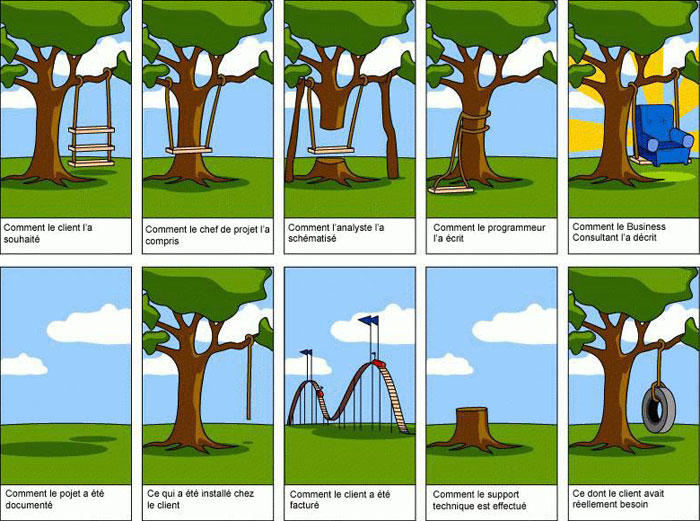
\includegraphics[width=16cm]{images/projet_info.jpg}
	\caption{Allégorie d'un projet informatique}
	\label{projet_info}
\end{figure}

\paragraph{}Par ailleurs, plusieurs séances peuvent avoir lieu tout au long du projet, afin de vérifier si les besoins ont évolués et si le développement actuel est effectivement en accord avec ceux-ci. Les utilisateurs aideront aussi l'équipe de recherche et développement à juger de la pertinence des solutions apportées.
\paragraph{}
D'un point de vue du développement, on notera que ce type de conception s'accorde parfaitement avec une méthodologie AGILE, et notamment la méthode SCRUM qui consiste en de courtes périodes de développement entre lesquelles on met en relief l'avancement par rapport au projet global.
